\chapter{Attention That Pervades Life}

This chapter follows J. Krishnamurti's San Diego dialogue with Dr. Alan W. Anderson on meditation, attention, sleep, control, and desire. The source is not a blackboard lecture and no validated board images remain, so the mathematical material here is deliberately schematic: we use arrows, contrasts, and compact diagrams only to preserve the structure of the inquiry. The point is not to turn Krishnamurti into a formal theorist, but to make the logic of the conversation visible without losing its rhythm.

\section{Beginning Without A Method}

Anderson opens by placing the dialogue at the point reached in the previous conversation: they are ready to take up meditation. The expected question would be, What is the right form of meditation? Krishnamurti refuses that beginning. There are too many ready-made answers: Indian schools, Zen, Christian contemplative orders, Sufi practices, prayer, mantra, breathing, repetition, discipline, silence, fasting, and the authority of those who claim to have arrived.

The first move is therefore negative, but not merely dismissive. We must not ask which method is best until we have asked what meditation is. More exactly, Krishnamurti asks whether we can begin by saying that we do not know.

\begin{definition}[The starting point]
In this dialogue, not-knowing does not mean confusion or intellectual vacancy. It means freedom from inherited conclusions, from the authority of systems, and from the burden of another person's experience.
\end{definition}

The schematic form is simple:

\begin{equation}
\text{not-knowing}
\longrightarrow
\text{freedom from authority}
\longrightarrow
\text{inquiry}.
\end{equation}

This is the first important structure of the chapter. Meditation is not first a procedure to be learned. It begins as the clearing away of second-hand certainty.

\section{Tradition, Practice, And The Static Goal}

Krishnamurti next examines what is hidden inside practice. A mantra is repeated, a prayer is repeated, a breathing exercise is repeated, a discipline is followed, and the mind is told that through repetition it will arrive at truth, God, illumination, or enlightenment. Anderson sharpens the point by distinguishing an activity whose end lies outside itself from an activity whose end is intrinsic to the act.

We can write the traditional structure as

\begin{equation}
\text{practice}
\longrightarrow
\text{imagined goal}.
\end{equation}

The problem is not just that practice may be dull. The deeper problem is that the goal has already been projected. If truth is something one practices in order to reach, then the mind has already pictured it as ``over there.'' And if it is already over there, waiting to be reached, then it has been made fixed.

\begin{equation}
\text{practice toward truth}
\Rightarrow
\text{truth treated as fixed or static}.
\end{equation}

Krishnamurti's objection is precise. A static truth is already dead. The repeated method may quiet, train, or condition the mind, but it cannot discover what is living if the destination has been fixed in advance.

\subsection{Question \& Answer}

\paragraph{Question.}
If practice aims at truth, must truth be treated as fixed?

\paragraph{Answer.}
In the logic of this dialogue, yes. The moment practice is organized as a path to a known or promised destination, the destination has already been imagined. One practices toward an image, a conclusion, a state. That makes the so-called truth static before inquiry has even begun. Krishnamurti therefore shifts the question from ``How shall we meditate?'' to ``What is meditation?''

\begin{figure}
\centering
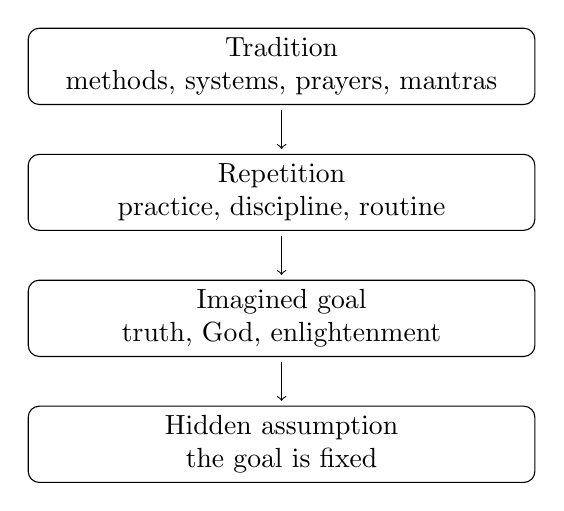
\begin{tikzpicture}[x=1cm,y=1cm]
\node[draw, rounded corners, align=center, text width=6.2cm] at (0,0)
{Tradition\\methods, systems, prayers, mantras};
\node[draw, rounded corners, align=center, text width=6.2cm] at (0,-1.6)
{Repetition\\practice, discipline, routine};
\node[draw, rounded corners, align=center, text width=6.2cm] at (0,-3.2)
{Imagined goal\\truth, God, enlightenment};
\node[draw, rounded corners, align=center, text width=6.2cm] at (0,-4.8)
{Hidden assumption\\the goal is fixed};
\draw[->] (0,-0.55) -- (0,-1.05);
\draw[->] (0,-2.15) -- (0,-2.65);
\draw[->] (0,-3.75) -- (0,-4.25);
\end{tikzpicture}
\end{figure}

This diagram is only a schematic reconstruction of the dialogue. There was no validated board diagram, but the sequence helps preserve the force of the argument.

\section{Meditation And The Whole Field Of Life}

Once the inherited paths have been put aside, Krishnamurti asks the first test question: is meditation divorced from daily living? The question is not decorative. It is the pivot of the dialogue. Daily living means conduct, desire, ambition, greed, envy, competition, imitation, conformity, sensuous appetite, sexual appetite, pleasure, anxiety, fear, death, and relationship. If meditation is apart from all this, then it becomes an escape from the very life it claims to illuminate.

We can state the contrast as

\begin{align}
\text{meditation} &\neq \text{escape from life},\\
\text{meditation} &\supset
\{\text{conduct}, \text{desire}, \text{fear}, \text{pleasure},
\text{death}, \text{relationship}, \text{work}\}.
\end{align}

The symbol \(\supset\) is not meant as formal set theory. It marks Krishnamurti's insistence that meditation must include the whole field, or it has no meaning. If meditation is only a period of withdrawal, an hour of repetition, or a private inward refuge, then it is still one more fragment.

Anderson's religious reflections belong here as part of the dialogue's movement. He brings in Christian prayer, the Jesus Prayer, and scriptural language about path and light. Krishnamurti's answer is not to argue theology. He keeps returning to the structure: repetition conditions the mind; belief carries tradition; a path assumes a fixed endpoint; meditation, if it is real, cannot be separated from living.

\section{Seeing The False And The Fragmented}

The next move is from tradition to perception. Krishnamurti does not say that one should condemn tradition because another authority has declared it false. He says the false must be seen. The eyes must look without prejudice and without reaction. Then the falseness of a thing is revealed in the seeing itself.

\begin{equation}
\text{perception without prejudice}
\longrightarrow
\text{the false seen as false}.
\end{equation}

The test remains practical. A person may claim truth, wisdom, love, or illumination, but Krishnamurti asks: has there been a change in conduct? Is there freedom from fear, ambition, greed, envy, and the desire for success? If not, the claim is a game.

This leads directly to fragmentation. Meditation includes the whole field of existence, so it cannot leave untouched the social divisions in which a human being hides: artist, businessperson, politician, priest, scholar, scientist. Krishnamurti does not analyze these as professions in a sociological sense. He treats them as outward expressions of an inward division.

\begin{equation}
\text{fragmented human being}
\longrightarrow
\{\text{artist}, \text{businessperson}, \text{politician},
\text{priest}, \text{scholar}, \text{scientist}\}.
\end{equation}

\subsection{Question \& Answer}

\paragraph{Question.}
Can art, scholarship, or science be whole if the human being is fragmented?

\paragraph{Answer.}
In the terms of the dialogue, no. The artist may be unusually sensitive to beauty and nature, but if apart from that he remains inwardly divided, the artistic identity does not make him whole. Krishnamurti's order is exact: first there must be the total human being; then whatever is created or done may have beauty. Otherwise the field of work becomes another expression of fragmentation.

\begin{figure}
\centering
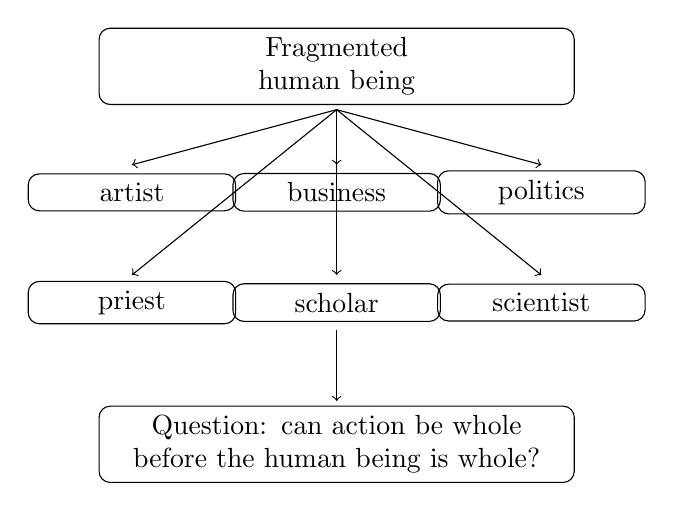
\begin{tikzpicture}[x=1cm,y=1cm]
\node[draw, rounded corners, align=center, text width=5.8cm] at (0,0)
{Fragmented\\human being};
\node[draw, rounded corners, align=center, text width=2.4cm] at (-2.6,-1.6) {artist};
\node[draw, rounded corners, align=center, text width=2.4cm] at (0,-1.6) {business};
\node[draw, rounded corners, align=center, text width=2.4cm] at (2.6,-1.6) {politics};
\node[draw, rounded corners, align=center, text width=2.4cm] at (-2.6,-3.0) {priest};
\node[draw, rounded corners, align=center, text width=2.4cm] at (0,-3.0) {scholar};
\node[draw, rounded corners, align=center, text width=2.4cm] at (2.6,-3.0) {scientist};
\node[draw, rounded corners, align=center, text width=5.8cm] at (0,-4.8)
{Question: can action be whole\\before the human being is whole?};
\draw[->] (0,-0.55) -- (-2.6,-1.25);
\draw[->] (0,-0.55) -- (0,-1.25);
\draw[->] (0,-0.55) -- (2.6,-1.25);
\draw[->] (0,-0.55) -- (-2.6,-2.65);
\draw[->] (0,-0.55) -- (0,-2.65);
\draw[->] (0,-0.55) -- (2.6,-2.65);
\draw[->] (0,-3.35) -- (0,-4.25);
\end{tikzpicture}
\end{figure}

The point is not to rank professions. It is to see that division is not healed by giving one fragment a noble name.

\section{Freedom As The Energy Of Inquiry}

The lecture now recaps its own movement. Systems, methods, gurus, authorities, beliefs, hopes: all these are burdens. Krishnamurti says that when they are put aside, the mind has no burden and is free to inquire. The claim is not merely verbal. He insists that he is speaking from what has been lived, not from borrowed phrases.

The working relation is

\begin{equation}
\text{discarding the burden of others}
\longrightarrow
\text{energy for inquiry}.
\end{equation}

This is a useful place to collect the derivation implicit in the first half of the lecture.

\begin{proof}
We begin with inherited meditation as method. Method implies repetition, discipline, and a projected end. A projected end makes truth into something already imagined. What is already imagined is static. Therefore the mind must put aside the method if it is to inquire into what is living. But putting aside method also means putting aside the authority, hope, and belief attached to it. When that burden falls away, the mind can begin from not-knowing. That not-knowing is humility, and that humility is the condition of real inquiry.
\end{proof}

This is not a mathematical proof in the formal sense. It is a disciplined reconstruction of the lecture's logic. It keeps the steps separate so that the next movement, into waking and sleep, does not appear arbitrary.

\section{Awake, Asleep, And The Past}

Having established that meditation covers the whole field of life, Krishnamurti now asks about sleep. But he does not begin with dreams. He begins with waking. What does it mean to be awake? Not merely awake to politics, economics, or social events, but awake inwardly and outwardly. Wakefulness is not a crisis, a shock, an incident, or a stimulated peak. If a stimulant is needed, one is already asleep.

The negative form is important:

\begin{align}
\text{stimulation} &\neq \text{wakefulness},\\
\text{fear or burden} &\Rightarrow \text{not awake}.
\end{align}

Anderson introduces the image of an animal's complete looking and complete sleeping. The example serves as a bridge, not as an argument from nature. Krishnamurti returns to the human question: is the past so alive that it dictates life in the present?

Here the distinction is delicate. The past is necessary as knowledge. One could not speak, work, remember a road, or use a skill without knowledge. But when the past covers the present, one is asleep now.

\begin{align}
\text{past as knowledge} &= \text{necessary},\\
\text{past covering present} &\Rightarrow \text{not awake}.
\end{align}

\subsection{Question \& Answer}

\paragraph{Question.}
Can the past function as knowledge without dominating the present?

\paragraph{Answer.}
That is precisely the question Krishnamurti wants to keep alive. Knowledge is necessary in practical affairs, but when the mind speaks and acts from the burden of past hurts, failures, depressions, conclusions, and experiences, the past has overflowed into the present. Then the present is not seen. The possible balance is that knowledge operates where it is needed, while awareness remains awake to what is taking place now.

A compact form is

\begin{equation}
\text{awareness} + \text{knowledge}
\longrightarrow
\text{no contradiction}.
\end{equation}

Anderson names this as a nexus between knowing and understanding. Krishnamurti accepts it as part of meditation, but he immediately continues the inquiry: if this is waking, what then is sleep?

\section{Dreams, Order, And The Rested Brain}

The question now becomes: what are dreams? Krishnamurti deliberately does not begin from what analysts, psychologists, or traditions say. He asks from the same ground as before: I do not know.

The sequence he gives is compact and important. If daily life is not watched, if its disorder is not understood, that disorder continues into sleep. The brain seeks order because without order it cannot function. Dreams and intimations may then be the brain's attempt to bring order during the night.

\begin{align}
\text{daily disorder unwatched}
&\longrightarrow
\text{disorder continues in sleep}
\longrightarrow
\text{dreams},\\
\text{daily disorder understood}
&\longrightarrow
\text{order}
\longrightarrow
\text{quiet sleep}
\longrightarrow
\text{rest}.
\end{align}

The claim should be kept in Krishnamurti's language. We should not expand it into neuroscience. The point is that order during the day changes the quality of sleep. If there is order through understanding disorder, the brain need not spend the night trying to secure order. Then sleep may be quiet, restful, and regenerative.

\subsection{Question \& Answer}

\paragraph{Question.}
Are all dreams merely unfinished disorder?

\paragraph{Answer.}
Anderson asks a related question about dreams that seem to point to a future event. Krishnamurti answers with an image: from high in the hills one may see two boats on a river moving toward a meeting point. This is not prediction in a mystical sense; it is a wider seeing. Anderson distinguishes that from subjective unfinished business. The main line remains: dreams, in the ordinary sense under discussion, continue the disorder that has not been understood during the day.

\begin{figure}
\centering
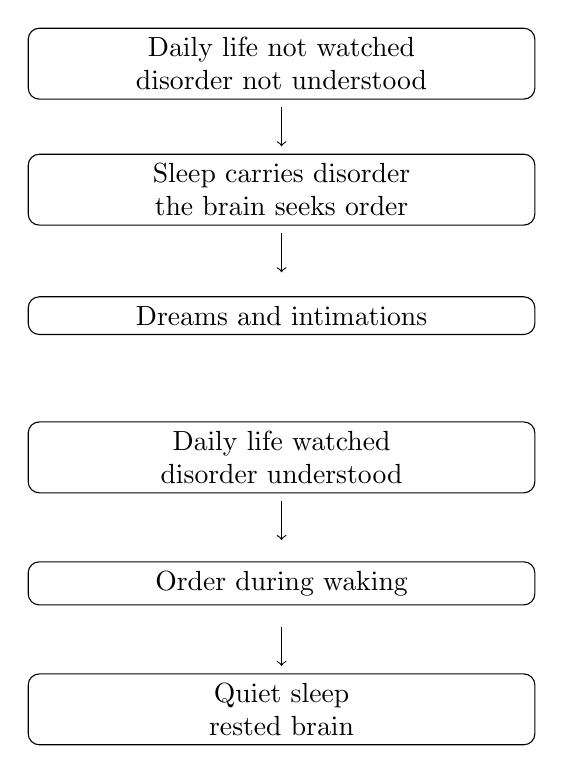
\begin{tikzpicture}[x=1cm,y=1cm]
\node[draw, rounded corners, align=center, text width=6.2cm] at (0,0)
{Daily life not watched\\disorder not understood};
\node[draw, rounded corners, align=center, text width=6.2cm] at (0,-1.6)
{Sleep carries disorder\\the brain seeks order};
\node[draw, rounded corners, align=center, text width=6.2cm] at (0,-3.2)
{Dreams and intimations};
\node[draw, rounded corners, align=center, text width=6.2cm] at (0,-5.0)
{Daily life watched\\disorder understood};
\node[draw, rounded corners, align=center, text width=6.2cm] at (0,-6.6)
{Order during waking};
\node[draw, rounded corners, align=center, text width=6.2cm] at (0,-8.2)
{Quiet sleep\\rested brain};
\draw[->] (0,-0.55) -- (0,-1.05);
\draw[->] (0,-2.15) -- (0,-2.65);
\draw[->] (0,-5.55) -- (0,-6.05);
\draw[->] (0,-7.15) -- (0,-7.65);
\end{tikzpicture}
\end{figure}

After this, the lecture asks whether the mind lives in this quality during the day. If it does not, Krishnamurti says, it is not meditation. The inquiry cannot be confined to the night.

\section{Control, Desire, And Flowering}

The final movement begins with another inherited command: all religions have said control. Control desire, control thought, control oneself. Krishnamurti again asks the prior question: what is control, and who is the controller?

The central identity is one of the sharpest statements in the dialogue:

\begin{equation}
\text{controller} = \text{controlled}.
\end{equation}

When one says, ``I must control my thought,'' the controller is itself a creation of thought. Thought is trying to control thought. One fragment attempts to dominate another fragment, and the result is still fragmentation.

\begin{equation}
\text{thought controls thought}
\Rightarrow
\text{fragmentation remains}.
\end{equation}

\subsection{Question \& Answer}

\paragraph{Question.}
Can there be a life of meditation without control?

\paragraph{Answer.}
Krishnamurti does not answer by permitting disorder. He asks whether order can exist without suppression. If intelligence is order, then the seeing itself is the doing; order does not have to be imposed by a controller. Control belongs to division. The question therefore becomes concrete in the field of desire.

Desire arises in a sequence:

\begin{equation}
\text{seeing}
\longrightarrow
\text{contact}
\longrightarrow
\text{sensation}
\longrightarrow
\text{desire}.
\end{equation}

Once desire is present, Krishnamurti distinguishes three movements:

\begin{equation}
\text{desire}
\longrightarrow
\{\text{suppression},\ \text{yielding},\ \text{flowering under watchfulness}\}.
\end{equation}

To suppress desire is another form of control. To yield to it fragments life into getting and losing. The third possibility is neither indulgence nor resistance: let desire come, flower, and be watched. In that watching, without choice, without suppression, without yielding, the flowering itself is the ending of that desire.

\begin{equation}
\text{desire observed without control}
\longrightarrow
\text{flowering}
\longrightarrow
\text{ending}.
\end{equation}

This is the lecture's closing image. Anderson recognizes the plant metaphor and asks to continue it in the next conversation. Krishnamurti agrees: meditation has not been finished. There is much more involved.

\section{Summary}

The chapter's movement is a disciplined clearing. Meditation is not first a method, a repetition, a prayer, a system, or a path to a projected goal. To begin there is to make truth fixed before inquiry starts. Krishnamurti begins instead with not-knowing, which frees the mind from inherited burdens.

From there the inquiry widens. Meditation must include the whole field of living: conduct, desire, fear, pleasure, death, relationship, work, art, and the fragmented roles of culture. It must also include waking and sleep. The past is necessary as knowledge, but when it covers the present it puts the mind to sleep. Dreams continue disorder when daily disorder has not been understood; order during the day permits quiet sleep and rest.

The final question is control. If the controller is the controlled, control is one fragment acting on another. The inquiry therefore moves to desire, not as something to be cut off or obeyed, but as a movement to be watched in its flowering. The chapter ends where the dialogue ends: not with a completed doctrine of meditation, but with attention opened further.